\section{Driven cavity problem}
The driven cavity problem consists in a two-dimensional cavity with an incompressible fluid. The upper wall of the cavity moves at a given velocity, as shown in figure \ref{DrivenCavityImg}. The aim of the problem is to obtain the distribution of velocities inside the cavity.
\begin{figure}
	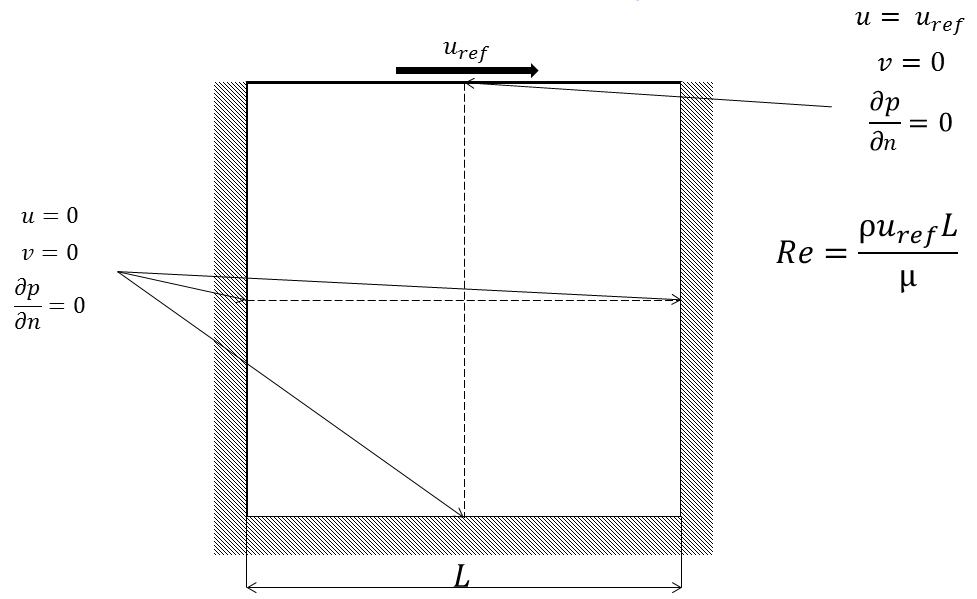
\includegraphics[scale=0.6]{DrivenCavity/DrivenCavity}
	\caption{General scheme of the driven cavity problem}
	\label{DrivenCavityImg}
\end{figure}

The equations to be solved are the conservation of mass and the conservation of momentum:
\begin{equation}
\begin{aligned}
\nabla\cdot=0 \\
\rho\frac{\partial\vec{v}}{\partial t}+\rho\left(\vec{v}\cdot\nabla\right)\vec{v}=-\nabla p+\mu\nabla^{2}\vec{v}
\end{aligned}
\end{equation}

\section{Fractional step method}
According to the Helmholtz-Hodge theorem, it is possible to decompose any vector in a divergence-free vector parallel to the boundary and a gradient field, and this decomposition is unique \cite{CTTC}.
Assuming constant density and viscosity, the Navier-Stokes equation can be rewritten as:
\begin{equation}
\rho\frac{\partial\vec{v}}{\partial t}=R\left(\vec{v}\right)-\nabla p
\label{RNSFSM}
\end{equation}
where $R\left(\vec{v}\right)=-\rho\left(\vec{v}\cdot\nabla\right)\vec{v}+\mu\nabla^{2}\vec{v}$.
Integrating the equation \ref{RNSFSM} over time:
\begin{equation}
\rho\frac{\vec{v}^{n+1}-\vec{v}^{n}}{\Delta t}=R^{n+\frac{1}{2}}\left(\vec{v}\right)-\nabla p^{n+1}
\end{equation}
However, the term $R^{n+\frac{1}{2}}\left(\vec{v}\right)$ is not easy to evaluate. To do so, the Adams-Bashforth second-order scheme is used:
\begin{equation}
R^{n+\frac{1}{2}}\left(\vec{v}\right)\approx\frac{3}{2}R\left(\vec{v^{n}}\right)-\frac{1}{2}R\left(\vec{v}^{n-1}\right)
\end{equation}
Applying the Helmholtz-Hodge Theorem, the intermediate velocity is easily obtained:
\begin{equation}
\vec{v}^{P}=\vec{v}^{n+1}+\frac{\Delta t}{\rho}\nabla p^{n+1}
\label{IntermediateVelocity}
\end{equation}
Introducing this expression to the integrated equation:
\begin{equation}
\rho\frac{\vec{v}^{P}-\vec{v}^{n}}{\Delta t}=R^{n+\frac{1}{2}}\left(\vec{v}\right)
\label{IntermediatewithR}
\end{equation}
And finally, applying the divergence to the expression of the intermediate velocity $\vec{v}^{P}$ \ref{IntermediateVelocity}, the Poisson equation is obtained:
\begin{equation}
	\nabla\cdot\vec{v}=\frac{\Delta t}{\rho}\nabla^{2}p
	\label{Poisson}
\end{equation}
With all these expressions the fractional step method (FSM) can be finally implemented, following the next scheme:
\begin{enumerate}
	\item Evaluate $R^{n+\frac{1}{2}}\left(\vec{v}\right)$.
	\item Calculate the intermediate velocity with equation \ref{IntermediatewithR}.
	\item Calculate the pressure $p^{n+1}$ from the Poisson equation \ref{Poisson} using a linear solver.
	\item Calculate the velocity at the next time step with equation \ref{IntermediateVelocity}.
\end{enumerate}
However, this method can be problematic if the mesh of the problem is not correctly implemented. To avoid having solutions with no physical sense, it is important to use staggered meshes or collocated meshes.

\section{Discretization}
To avoid convergence problems or incorrect solutions, the staggered meshes are used. As shown in figure \ref{staggered}, in a two-dimensional case there are 3 control volumes, one for each variable: $p_{P}$, $u_{P}$ and $v_{P}$. They are coloured in black, red and green respectively.
\begin{figure}
	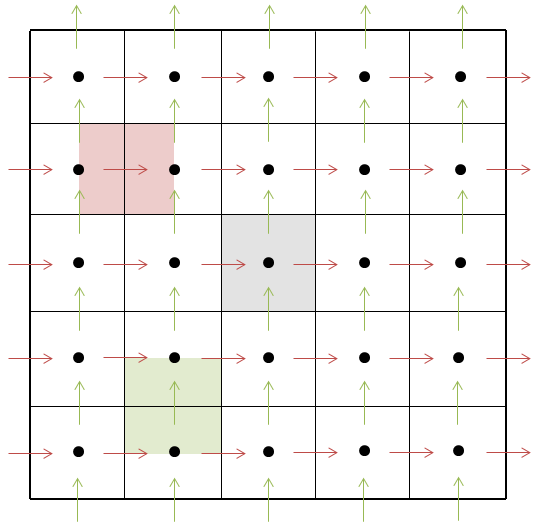
\includegraphics[scale=0.8]{DrivenCavity/staggered}
	\caption{Staggered meshes (2D)}
	\label{staggered}
\end{figure}
Knowing the space discretization of the domain, the discretized Poisson equation can be calculated. Integrating the expression over the domain and applying the divergence theorem, the following expression can be easily obtained:
\begin{equation}
\frac{p_{E}^{n+1}-p_{P}^{n+1}}{d_{EP}}A_{e}+\frac{p_{N}^{n+1}-p_{P}^{n+1}}{d_{NP}}A_{n}-\frac{p_{P}^{n+1}-p_{W}^{n+1}}{d_{WP}}A_{w}-\frac{p_{P}^{n+1}-p_{S}^{n+1}}{d_{SP}}A_{s}=\frac{1}{\Delta t}\left[\left(\rho u^{P}\right)_{e}A_{e}+\left(\rho v^{P}\right)_{n}A_{n}-\left(\rho u^{P}\right)_{w}A_{w}-\left(\rho v^{P}\right)_{s}A_{s}\right]
\end{equation}
Rewriting the equation using discretization coefficients:
\begin{equation}
	a_{P}p_{P}^{n+1}=a_{E}p_{E}^{n+1}+a_{W}p_{W}^{n+1}+a_{N}p_{N}^{n+1}+a_{S}p_{S}^{n+1}+b_{P}
\end{equation}
where
\begin{equation}
a_{P}=a_{E}+a_{W}+a_{N}+a_{S}
\end{equation}
\begin{equation}
a_{E}=\frac{A_{e}}{d_{EP}}
\end{equation}
\begin{equation}
a_{W}=\frac{A_{w}}{d_{WP}}
\end{equation}
\begin{equation}
a_{N}=\frac{A_{n}}{d_{NP}}
\end{equation}
\begin{equation}
a_{S}=\frac{A_{s}}{d_{SP}}
\end{equation}
\begin{equation}
b_{P}=-\frac{1}{\Delta t}\left[\left(\rho u^{P}\right)_{e}A_{e}+\left(\rho v^{P}\right)_{n}A_{n}-\left(\rho u^{P}\right)_{w}A_{w}-\left(\rho v^{P}\right)_{s}A_{s}\right]
\end{equation}

\section{Boundary conditions}
It is necessary to impose the conditions defined by figure \ref{DrivenCavityImg}. These boundary conditions modify the discretization coefficients in the boundary nodes.
There are two types of conditions: the prescribed velocity, and the boundary layer conditions. The last ones are defined by assuming that the pressure gradient normal to the wall is 0. For example, in the left wall:
\begin{equation}
	\frac{\partial p}{\partial x}\approx\frac{p_{E}-p_{P}}{\Delta x}=0
\end{equation}
\begin{equation}
P_{P}=p_{E}
\end{equation}
The prescribed velocity is defined using a similar approach. It is assumed that $u_{P}^{n+1}=u^{P}$. To obtain this solution, the pressure gradient has to be equal to zero, so the same expression as in the boundary layer conditions is obtained.
\begin{table}
	\centering
	\begin{tabular}{ |c|c|c|c|c| }
		\hline
		Coefficients & Top & Bottom & Left & Right \\ \hline
		$a_{E}$ & 1 & 0 & 1 & 0 \\ \hline
		$a_{W}$ & 0 & 0 & 0 & 1 \\ \hline
		$a_{N}$ & 0 & 1 & 0 & 0 \\ \hline
		$a_{S}$ & 0 & 0 & 0 & 0 \\ \hline
		$a_{P}$ & 1 & 1 & 1 & 1 \\ \hline
	\end{tabular}
\caption{Discretization coefficients in the boundary}
\end{table}

